\documentclass[12pt]{article}
\usepackage[margin=1in]{geometry}
\usepackage{blindtext}
\usepackage{ragged2e}
\usepackage{csquotes}
\usepackage{graphicx}
\usepackage{rotating}
\usepackage{wrapfig}
\usepackage{subcaption}
\usepackage{float}
\usepackage{amsmath,amsthm,amssymb}
\usepackage{setspace}
\usepackage{lscape}
\usepackage{caption}
\usepackage{subcaption}
\usepackage[utf8]{inputenc}
\usepackage{threeparttable}
\usepackage{pdflscape}
\usepackage{xcolor}
\usepackage{pgfplots}
\usepackage{tikz}
\usepackage{soul}
\usepackage{natbib}

\begin{document}

\begin{center}
Kaleigh Strohl \\
ECON833: Problem Set 9 \\
Fall 2021
\end{center}

\noindent The code Angela, Paul, and I worked on ended up not working, which is really disappointing. The .py files attached are our closest attempt - I believe something is wrong with the dimensions of our functions and/or how the FOC returns are defined. The resulting arrays should be \(2S-1\) in length, which would be 159 given our parameters, but ours are length 2. Additionally, Python is telling us they should be length 161, so we have a lot that isn't lining up correctly here.\\\\
\noindent If our code had worked, the SS solver should have returned the optimal values of \(r\) that ensures a steady state in the economy. We would have been able to plot the corresponding trends of consumption(\(c\)), savings(\(b\)), and labor(\(n\)) over time. The respective plots for consumption, savings, and labor should look similar to what was shown in the notes: 
\begin{figure}[h]
	\begin{subfigure}[b]{0.45\textwidth}
		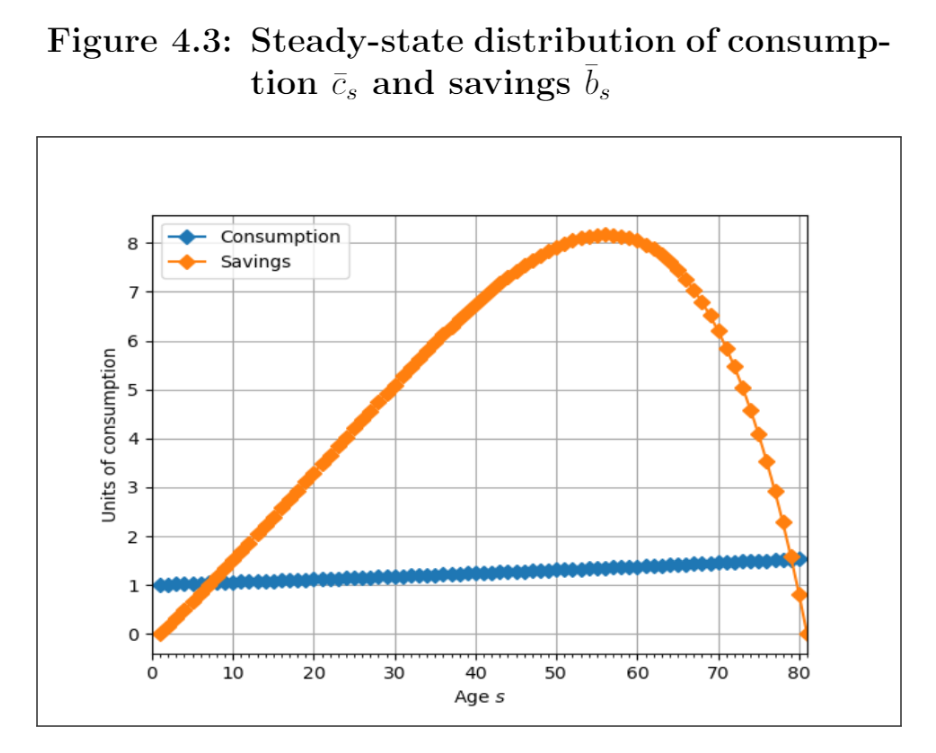
\includegraphics[width=\textwidth]{examplefig_c_s.png}
		\caption{Example: Consumption and Savings}
	\end{subfigure}
	\hfill
	\begin{subfigure}[b]{0.45\textwidth}
		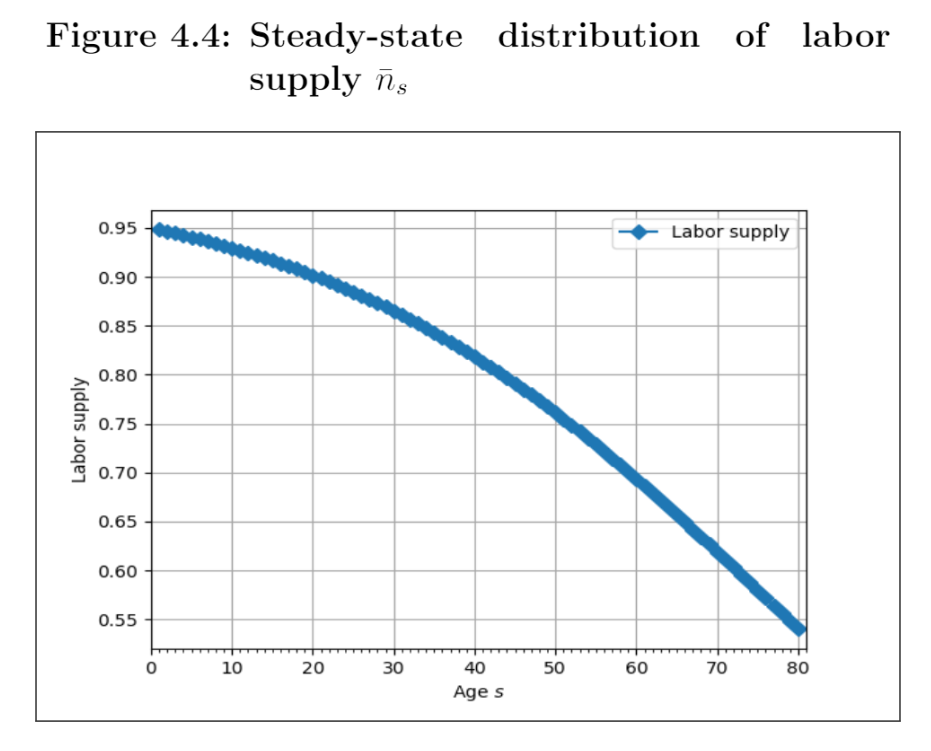
\includegraphics[width=\textwidth]{examplefig_L.png}
		\caption{Example: Labor}
	\end{subfigure}
\end{figure}

\noindent We see that consumption is gradually increasing over time. Savings initially increase, but then hit a peak and decrease as the stock of savings are depleted before time ends. Labor decreases over time (meaning leisure increases).
\end{document}